\documentclass[tikz,border=6pt]{standalone}
\usepackage[T1]{fontenc}
\usepackage[utf8]{inputenc}
\usepackage{pgfplots}
\usepgfplotslibrary{groupplots}
\usetikzlibrary{calc}
\pgfplotsset{compat=1.18}
\begin{document}
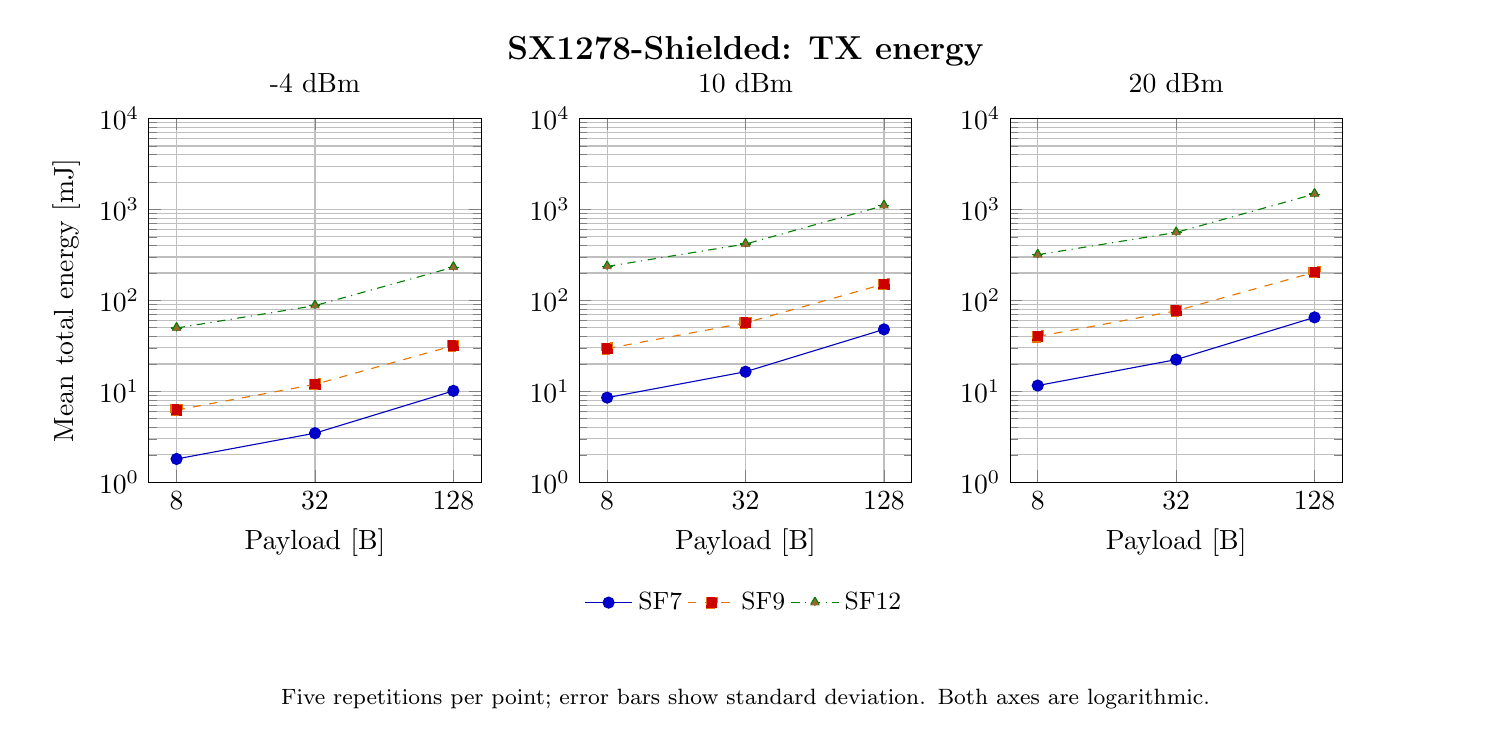
\begin{tikzpicture}
\begin{groupplot}[/pgf/number format/use comma, group style={group size=3 by 1, horizontal sep=1.25cm},
  width=5.8cm,height=6.2cm,xmode=log,log basis x=2,ymode=log,log basis y=10,ymin=1,ymax=10000,
  xtick={8,32,128},xticklabels={8,32,128},grid=both,xlabel={Payload [B]},
  legend style={draw=none,fill=none,font=\small,at={(0.5,-0.27)},anchor=north,legend columns=-1}]
% TX energy
\nextgroupplot[title={-4 dBm},ylabel={Mean total energy [mJ]}]
\addplot+[blue!75!black,solid,mark=*,error bars/.cd,y dir=both,y explicit] coordinates {(8,1.80249122) +- (0,0.00347503106) (32,3.46384036) +- (0,0.00463016193) (128,10.1133266) +- (0,0.0151384104)};
\addplot+[orange!90!black,dashed,mark=square*,error bars/.cd,y dir=both,y explicit] coordinates {(8,6.22762691) +- (0,0.00794026019) (32,11.9168782) +- (0,0.0228875708) (128,31.785535) +- (0,0.0322128404)};
\addplot+[green!50!black,dashdotted,mark=triangle*,error bars/.cd,y dir=both,y explicit] coordinates {(8,49.6683261) +- (0,0.0764929726) (32,87.5989263) +- (0,0.0451124662) (128,231.905493) +- (0,0.146611164)};
\nextgroupplot[title={10 dBm}]
\addplot+[blue!75!black,solid,mark=*,error bars/.cd,y dir=both,y explicit] coordinates {(8,8.52262055) +- (0,0.000729523185) (32,16.4284343) +- (0,0.001572405) (128,48.0138967) +- (0,0.0203379913)};
\addlegendentry{SF7}
\addplot+[orange!90!black,dashed,mark=square*,error bars/.cd,y dir=both,y explicit] coordinates {(8,29.5441058) +- (0,0.014993362) (32,56.619017) +- (0,0.0145411931) (128,151.32233) +- (0,0.0391580031)};
\addlegendentry{SF9}
\addplot+[green!50!black,dashdotted,mark=triangle*,error bars/.cd,y dir=both,y explicit] coordinates {(8,236.323977) +- (0,0.0616952711) (32,416.961556) +- (0,0.0831643644) (128,1104.34796) +- (0,0.342109953)};
\addlegendentry{SF12}
\nextgroupplot[title={20 dBm}]
\addplot+[blue!75!black,solid,mark=*,error bars/.cd,y dir=both,y explicit] coordinates {(8,11.5706367) +- (0,0.0325694736) (32,22.3185974) +- (0,0.0503614631) (128,65.108905) +- (0,0.259756251)};
\addplot+[orange!90!black,dashed,mark=square*,error bars/.cd,y dir=both,y explicit] coordinates {(8,40.1096596) +- (0,0.138091313) (32,76.7688434) +- (0,0.237188675) (128,204.035026) +- (0,0.570118976)};
\addplot+[green!50!black,dashdotted,mark=triangle*,error bars/.cd,y dir=both,y explicit] coordinates {(8,317.963839) +- (0,0.941609621) (32,558.877771) +- (0,1.53508764) (128,1479.71917) +- (0,2.17294431)};
\end{groupplot}
\node[font=\bfseries\large] at ($(group c2r1.north)+(0,0.85cm)$) {SX1278-Shielded: TX energy};
\node[font=\footnotesize,align=center,text width=18cm] at ($(group c2r1.south)+(0,-2.75cm)$) {Five repetitions per point; error bars show standard deviation. Both axes are logarithmic.};
\end{tikzpicture}
\end{document}
